\documentclass{article}
\usepackage{authblk}
\usepackage{acro}
\usepackage{amsmath}
\usepackage{amsfonts}
\usepackage{caption}
\usepackage{ccaption}
\usepackage[margin=20truemm]{geometry}
\usepackage[dvipdfmx]{graphicx}
\usepackage{hyperref}
\usepackage{url}

\title{\empty}
\author{\empty}
\date{\empty}

\DeclareCaptionLabelFormat{supplemental}{\textbf{Figure S#2}}
\captionsetup[figure]{labelformat=supplemental}

\urlstyle{same}

\begin{document}

\maketitle

\section*{Appendix}
\subsection*{Supplemental Information}
\subsubsection*{Cell clusters vs cells classes}
A cell cluster refers to a stochastic chunk of samples neighbouring each other in the data space or spacific feature 
space designed via the data analysis. Hence, cell clusters can be defined without introducing GRNs or eigen-cascades. 
Contrary, a cell class refers a set of samples, which can be treated identical, and their biological features 
characterized with the eigen-cascades. In this context, what is identical can be defined by a clustring function (i.e., 
a mapping between samples and the clusters that they belong to) of choice. Therefore, the term cell class 
emphasizes the randomness of a cell cluster and always tagged with the concept of eigen-cascades. On the other hand, 
we use cell cluster to refer some data-driven groups of cells in a more neutral nuance.

\newpage
\subsection*{Supplemental Figures}
\begin{figure}[htb]
  \centering
  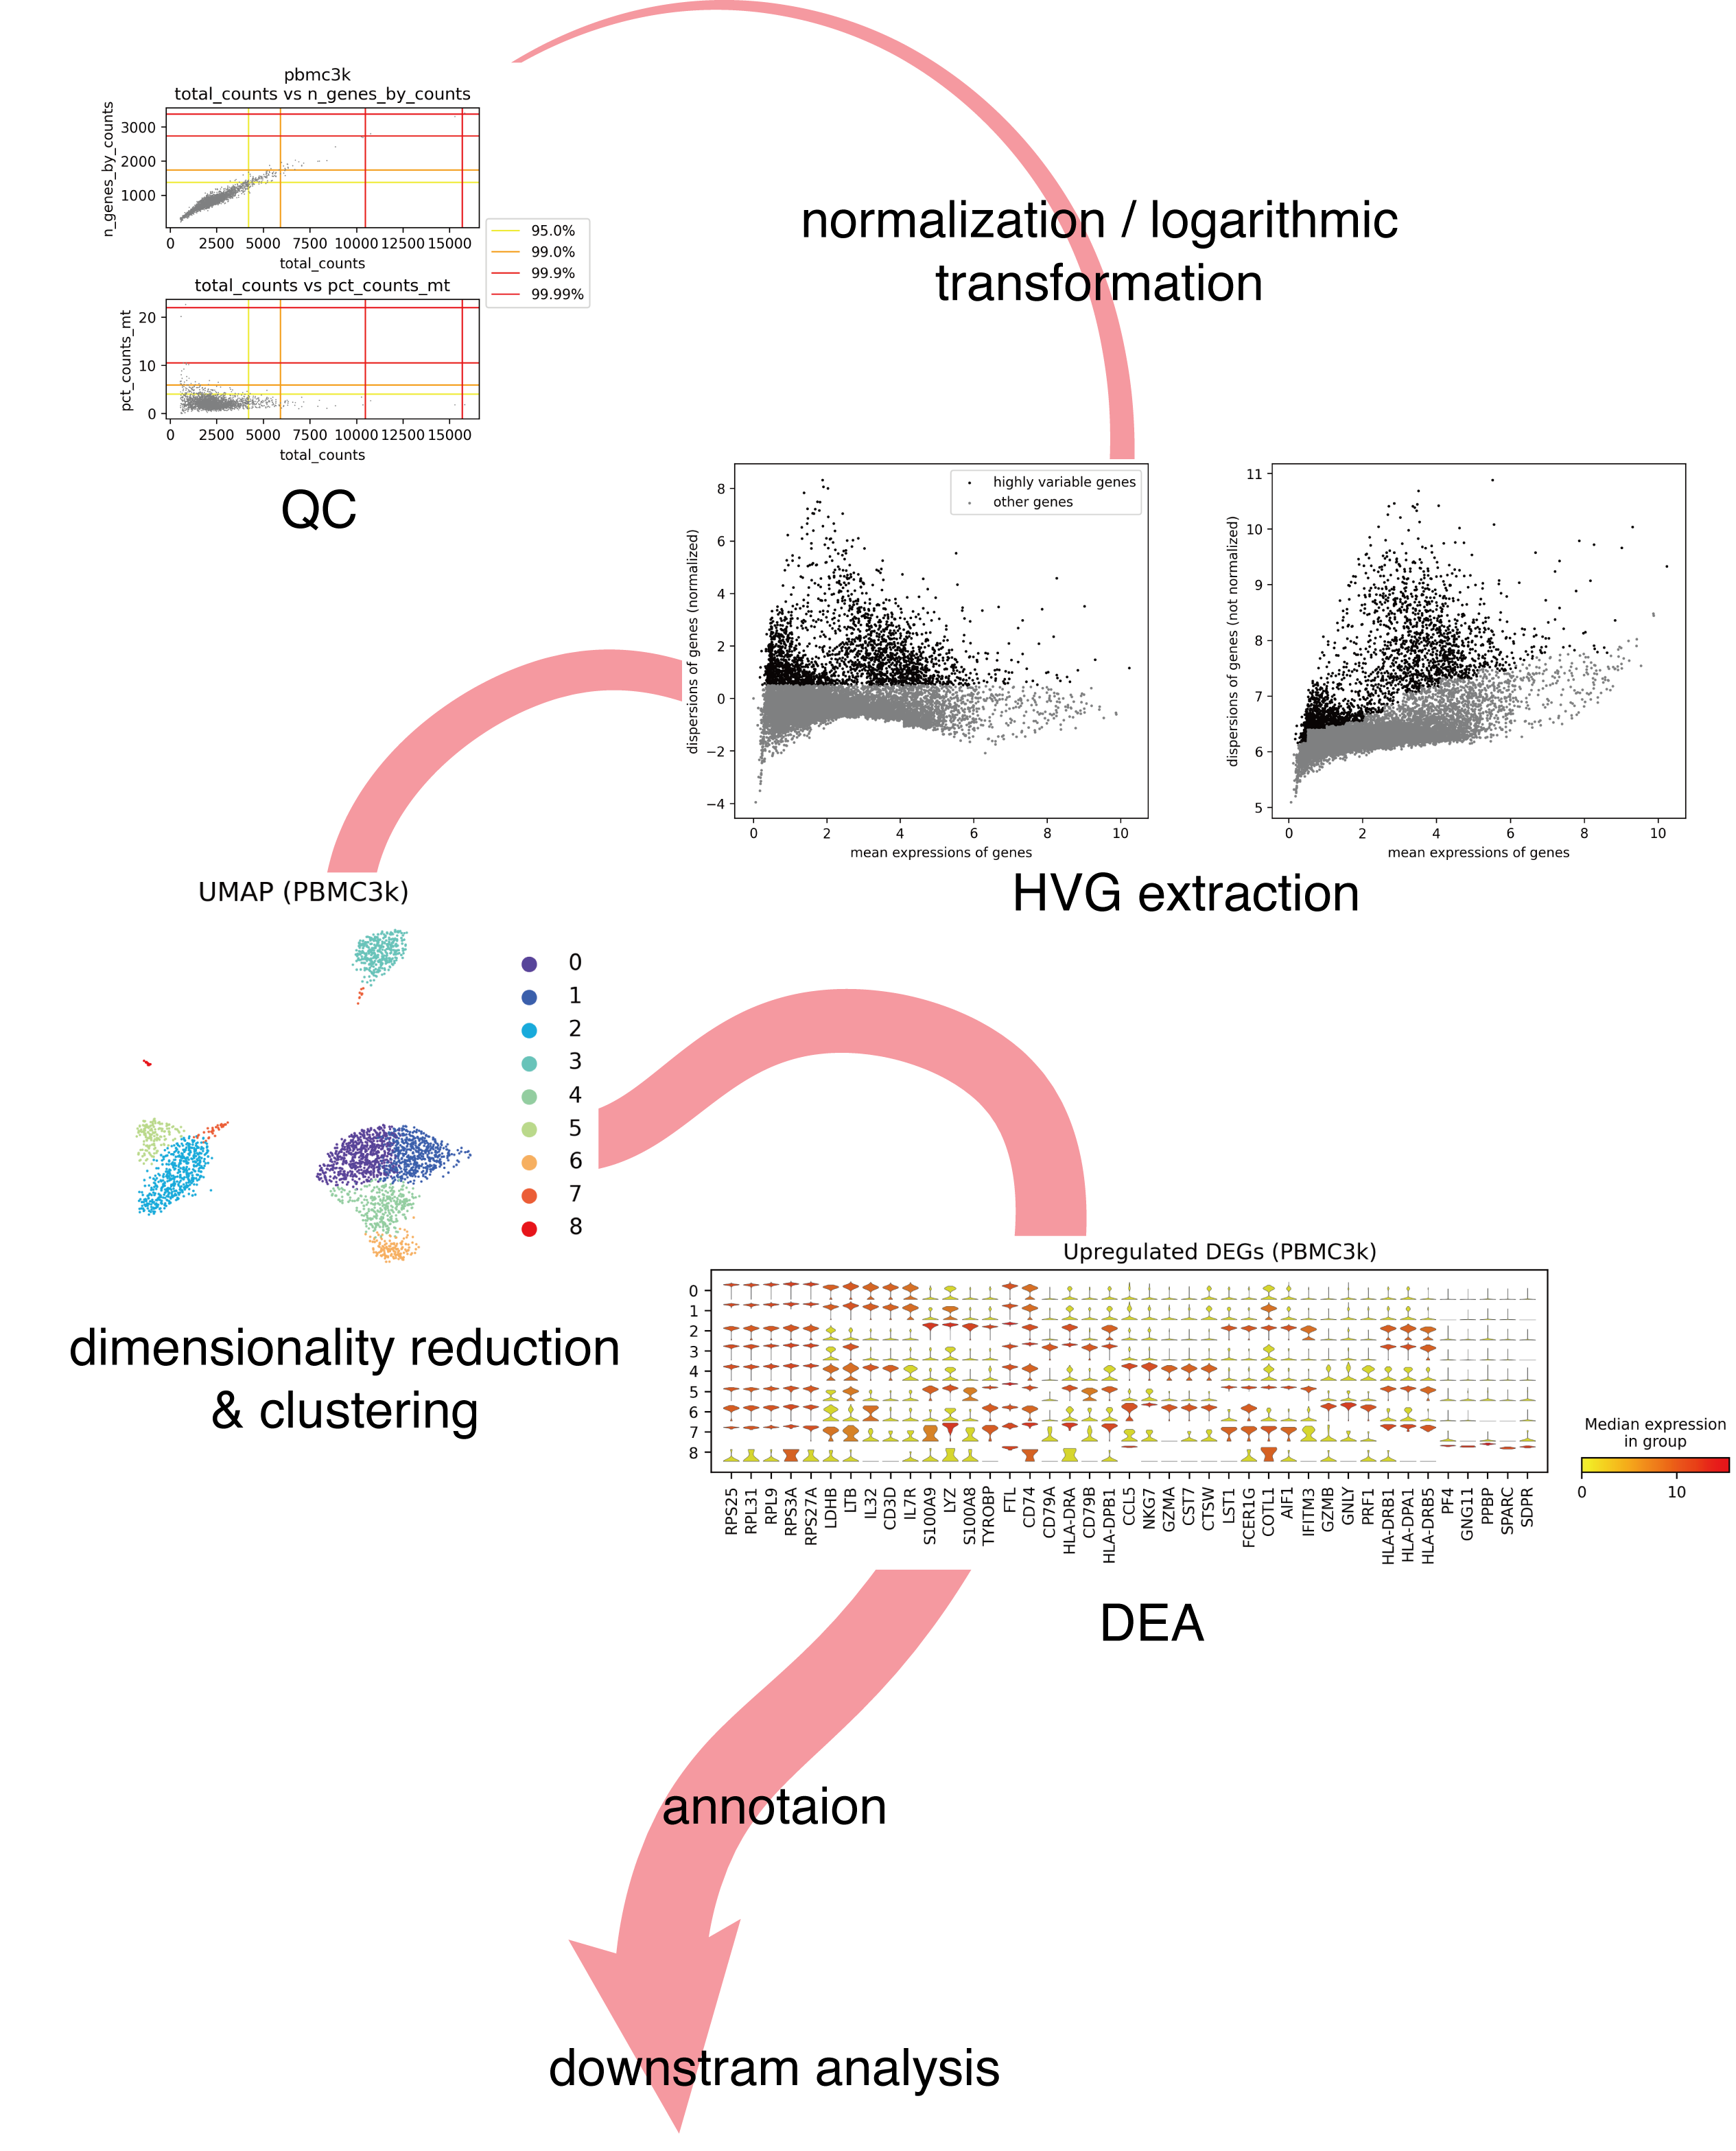
\includegraphics[scale=0.6]{./figs/exported/figure_s1.png}
  \caption{Gene expression patterns of clusters in PBMC3k}
  \legend{
    \textbf{A}: Violin plot of DEGs of the clusters (top 5 for each). 
    \textbf{B}: GRNs of the clusters. GRNs in a row share the same set of genes
    (DEGs of the subjective clusters) for the nodes
  }
  \label{fig_s1}
\end{figure}

\end{document}
